\section{问题三：组合预报与日内调整}
\subsection{统一发布相位的组合预报}
零点计划层以及各调整时刻$r\in\{6,12,18\}$均采用
\begin{equation}
\widetilde P^{(r)}_{d,t}=
\left[\lambda\widehat P^{\,\mathrm{off},r}_{d,t}
+(1-\lambda)\widehat P^{\,\mathrm{hist}}_{d,t}-m\Delta t\right]_+,
\quad \lambda=0.7.
\label{eq:mix}
\end{equation}
官方预报使用对应发布时刻的曲线，历史项与问题二一致；负荷继续使用因果历史预测和$\kappa=1.02$修正。第二日尚无对应零点官方预报，使用零点可得的历史外推。
采用相同组合形式的目的，是使日内更新仅反映新信息，而不同时改变预测构造。

\subsection{调整费用的等价表达}
对某个尚未执行的槽，设原计划为$x^0$、最终调整量为$x^a$。
当$x^a\leq x^0$，购电加违约费用为$px^a+0.5p(x^0-x^a)$；
当$x^a>x^0$，费用为$px^0+1.5p(x^a-x^0)$。二者统一为
\begin{equation}
g(x^a;x^0)=px^a+0.5p|x^a-x^0|.
\label{eq:adjustcost}
\end{equation}
因此不能将原计划费用再完整相加，否则会重复计费。
引入$y\leq x^0,\ y\leq x^a,\ y\geq0$，则
$g=1.5px^a-py+0.5px^0$在最优时成立。
最后一项对调整决策是常数，可在求解时省略，但费用统计必须恢复。

\subsection{名义调整与日末参考}
每次新预报发布后，以当前实际SOC初始化剩余时段规划，已执行时段不再修改。
零点两日规划产生当日末的参考电量$E^{\rm ref}_{d,T}=E^{\rm plan}_{d,144}$。
当前日内调整LP保留
\begin{equation}
E^{\rm adj}_{d,T}=E^{\rm ref}_{d,T}
\label{eq:adjterminal}
\end{equation}
作为规划连接条件；该参考由每日预测、价格与日初状态共同决定，并非恒定6000 kWh。
实际执行仍用式\eqref{eq:discharge}--\eqref{eq:charge}，不强制到达此参考。
因而必须区分“规划采用动态日末参考”和“实际日末电量自由”。
这种分层连接保留了次日储能需求的部分信息，但日内层尚未直接重算完整两日窗口，属于模型近似。

\subsection{联合场景候选扩展}
为检验随机规划能否进一步降低短缺风险，先构造一个对冲候选扩展。
在6时和12时，从目标日之前的最近90天中选择残差池；其中同月样本达到14天时优先使用同月样本。
对历史日$j<d$，用其对应发布时刻的名义预测构造联合残差
\begin{equation}
R^L_{j,t}=L_{j,t}-\widetilde L_{j,t},\qquad
R^{P,r}_{j,t}=P_{j,t}-\widetilde P^{(r)}_{j,t}.
\label{eq:residual}
\end{equation}
同一场景的负荷和光伏取自同一天，并保留整段曲线。
每次调整使用$S=40$个等权情景，包含1个名义情景及39个有放回重采样情景；两次调整共抽样78个残差日索引，并不表示每次有78个场景。

不同情景共享调整量$x^a$，各自拥有充放电、弃电、储能与紧急补救变量。
对剩余时段集合$\mathcal T_r$，求解
\begin{equation}
\min\ \sum_{t\in\mathcal T_r}(1.5p_tx^a_t-p_ty_t)
+\frac1S\sum_{s=1}^S\sum_{t\in\mathcal T_r}
\left[5p_te^s_t+\varepsilon(c^s_t+q^s_t)\right],
\label{eq:scenarioobj}
\end{equation}
约束为各情景下的能量平衡、SOC动态、容量与功率界限，以及式\eqref{eq:adjterminal}和$y$的线性化约束。
目标中的$1/S$不可省略，否则情景数增加等价于人为提高紧急费权重。
18时采用名义剩余时段调整；这是一项计算与信息价值折中，并不意味着18时以后完全没有负荷不确定性。

场景内的补救轨迹仅服务于计划评价，其拥有的整段情景信息不等于实际执行可提前获知未来。
候选扩展的实现费用也一律用逐槽因果执行回放计算：
\begin{equation}
C_3=\sum_{d,t}\left[p_tx^a_{d,t}+0.5p_t|x^a_{d,t}-x^0_{d,t}|+5p_te_{d,t}\right].
\label{eq:q3cost}
\end{equation}
正式方案则不求解式\eqref{eq:scenarioobj}，在每个发布时刻只按最新组合名义预测调整剩余计划。
这样既保留相同的信息结构和动态日末参考，又消除了场景抽样及完整情景补救带来的额外保守性。
\subsection{整体表现与指定日期结果}
正式主方案334天总费用1347.1万元，其中计划费1290.5万元、调整净额25.2万元、紧急费31.4万元。
此处调整净额定义为$\sum[g(x^a;x^0)-px^0]$，不是绝对偏差费本身。
与官方预报无调整基线1464.5万元相比，费用降低8.01\%；与官方预报三点调整1357.5万元相比降低0.76\%。
图\ref{fig:q3compare}说明主要收益来自允许更新和调整，组合预测进一步小幅改善费用。
\begin{figure}[htbp]\centering
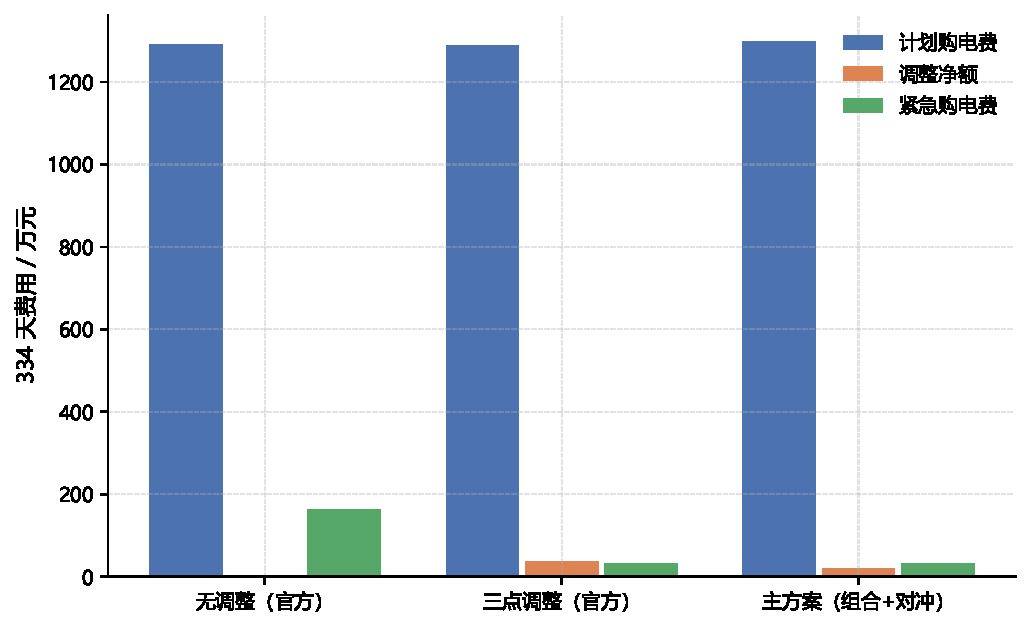
\includegraphics[width=.85\textwidth]{../../figures/Q3_策略费用对比.pdf}
\caption{问题三不同信息与调整策略的费用分解}\label{fig:q3compare}
\end{figure}
\begin{table}[htbp]\centering
\caption{问题三指定日期计划购电量与购电费}\label{tab:q3buy}
\small
\begin{tabular}{lrrrr}
\toprule
时段或指标 & 3月20日 & 6月21日 & 9月23日 & 12月21日 \\
\midrule
10:00-10:10 & 0.00 & 0.00 & 0.00 & 0.00 \\
12:00-12:10 & 567.21 & 0.00 & 419.53 & 966.15 \\
14:00-14:10 & 0.00 & 0.00 & 0.00 & 0.00 \\
16:00-16:10 & 618.29 & 187.98 & 586.23 & 811.78 \\
18:00-18:10 & 706.57 & 0.00 & 787.06 & 735.24 \\
20:00-20:10 & 0.00 & 0.00 & 0.00 & 0.00 \\
全天计划电量/kWh & 64357.79 & 40036.23 & 70612.27 & 96295.77 \\
全天计划购电费/元 & 39979.30 & 22282.70 & 43935.46 & 61825.34 \\
\bottomrule
\end{tabular}
\end{table}
\begin{table}[htbp]\centering
\caption{问题三指定日期调整购电量与购电费}\label{tab:q3adj}
\small
\begin{tabular}{lrrrr}
\toprule
时段或指标 & 3月20日 & 6月21日 & 9月23日 & 12月21日 \\
\midrule
10:00-10:10 & 0.00 & 0.00 & 0.00 & 0.00 \\
12:00-12:10 & 567.21 & 0.00 & 419.53 & 999.84 \\
14:00-14:10 & 0.00 & 0.00 & 0.00 & 0.00 \\
16:00-16:10 & 520.24 & 160.44 & 543.94 & 822.58 \\
18:00-18:10 & 706.57 & 0.00 & 787.06 & 735.24 \\
20:00-20:10 & 0.00 & 0.00 & 0.00 & 0.00 \\
调整后全天电量/kWh & 62231.04 & 40260.15 & 68561.04 & 96287.52 \\
买入及偏差费/元 & 40053.91 & 22874.05 & 43321.23 & 62209.20 \\
紧急购电费/元 & 20.44 & 0.00 & 43.00 & 74.30 \\
含紧急费总额/元 & 40074.34 & 22874.05 & 43364.23 & 62283.49 \\
\bottomrule
\end{tabular}
\end{table}
\begin{table}[htbp]\centering
\caption{问题三指定日期储能充放电与首末电量（kWh）}\label{tab:q3soc}
\footnotesize
\setlength{\tabcolsep}{4pt}
\begin{tabular}{lrrrrrrrr}
\toprule
 & \multicolumn{2}{c}{3月20日} & \multicolumn{2}{c}{6月21日} & \multicolumn{2}{c}{9月23日} & \multicolumn{2}{c}{12月21日}\\
区间 & 充电 & 放电 & 充电 & 放电 & 充电 & 放电 & 充电 & 放电 \\
\midrule
0:00-4:00 & 1292.66 & 122.05 & 447.73 & 200.31 & 1884.60 & 43.58 & 1956.07 & 276.70 \\
4:00-8:00 & 774.90 & 5841.05 & 525.84 & 2870.08 & 424.36 & 6752.50 & 1608.84 & 1579.87 \\
8:00-12:00 & 4175.67 & 2777.38 & 8988.07 & 0.00 & 5718.41 & 1896.62 & 5457.61 & 7155.69 \\
12:00-16:00 & 6164.61 & 260.50 & 0.00 & 0.00 & 5429.52 & 500.05 & 7167.18 & 2237.06 \\
16:00-20:00 & 233.47 & 5454.62 & 267.54 & 5481.91 & 188.48 & 5720.29 & 3.13 & 5687.61 \\
20:00-24:00 & 4089.80 & 3017.89 & 8635.18 & 2570.34 & 8474.10 & 2944.14 & 8405.16 & 2848.38 \\
0:00电量 & \multicolumn{2}{c}{9137.12} & \multicolumn{2}{c}{5246.06} & \multicolumn{2}{c}{8851.11} & \multicolumn{2}{c}{8728.51} \\
24:00电量 & \multicolumn{2}{c}{4780.15} & \multicolumn{2}{c}{9865.50} & \multicolumn{2}{c}{8917.34} & \multicolumn{2}{c}{8883.03} \\
\bottomrule
\end{tabular}
\end{table}
\begin{table}[htbp]\centering
\caption{问题三指定日期全部紧急购电事件}\label{tab:q3emerg}
\small
\begin{tabular}{ccr}
\toprule
日期 & 紧急购电时段 & 紧急购电量/kWh \\
\midrule
3月20日 & 20:30-20:40 & 2.9299 \\
6月21日 & 无 & 0.0000 \\
9月23日 & 20:20-20:30 & 6.3750 \\
12月21日 & 7:50-8:00 & 12.7909 \\
\bottomrule
\end{tabular}
\end{table}

表\ref{tab:q3buy}--\ref{tab:q3emerg}同时列出零点计划与调整后结果，便于区分承诺、实际执行与最终结算。
\subsection{消融检验与其他预报时刻}
\begin{table}[htbp]\centering
\caption{组合预报、对冲与信息一致性的消融结果}\label{tab:ablation}
\begin{tabular}{lrr}
\toprule
配置 & 总费用/万元 & 紧急费/万元\\\midrule
官方预报、三点调整、无对冲 & 1357.5 & 34.1\\
正式主方案：组合、三点调整、无对冲 & 1347.1 & 31.4\\
候选扩展：组合、三点调整及对冲 & 1349.2 & 33.6\\
计划组合、调整层仅官方且含对冲 & 1353.0 & 33.8\\
\bottomrule
\end{tabular}
\end{table}
表\ref{tab:ablation}表明，组合预报在无对冲结构下比单一官方预报降低10.4万元。
对冲扩展相对正式方案增加约2.1万元，且紧急费与紧急购电量均增加。
进一步按预先划分区间核算，开发期对冲仅低0.20万元，而冻结验证期无对冲低2.30万元；
因此这并非只按全年结果事后择优，留出证据同样不支持保留对冲。
据此正式方案删除对冲，将其保留为负结果；未来只有在新增独立极端样本并验证P95或CVaR收益后才考虑恢复。

对于题目提出的其他发布时刻，现有附件只提供四次预报，无法可靠计算新增时刻的实际收益。
可用“新增预报带来的期望紧急费节省，是否超过调整成本与获取成本”作为判据。
早晨或中午天气突变时提高预报频率可能有价值，但不能由现有结果宣称某个未观测时刻最优。
\questionconclusion{组合无对冲主方案费用1347.1万元，较官方无调整基线下降8.01\%；对冲在冻结验证期与全年均增费，故不进入正式策略。}
